\section{Fast computation of planned release-times}
We first show that a fixed relationship between variables $s_{jp}$ and $t_j$
can be assumed while looking for an optimal $(s,t)$.
Based on this, a problem $(P')$ is defined which can be solved instead of $(P)$.

\subsubsection{A tighter formulation}
Begin by rewriting (\ref{P-sjtj}) as $t_j \geq \max_p s_{jp} -w \,, \forall j \in V$.
Now, let $\Lambda$ denote the set of all feasible $(s,t)$ for problem $(P)$ and 
let $\Lambda^* \subseteq \Lambda$ be that part of the solution-space that 
only contains $(s,t)$ for which $t_j = \max_p s_{jp} - w$ for all $j$.

\begin{lemm}
	\label{lemm-Lambda}
	For every feasible $(s,t) \in \Lambda \setminus \Lambda^*$ 
	there exists $(s',t') \in \Lambda^*$ with equal objective value.
\begin{proof}
	Consider feasible $(s,t)$ with
 	$t_j = \max_p s_{j^*p} - w + c$ with  $c > 0$ for some $j^*$.
	Construct $t'$ by letting $t'_j = t_j$ for all $j \neq j^*$ and $t'_{j^*} = t_{j^*} - c = \max_p s_{j^*p} - w$.
	Trivially, if $(s,t)$ is feasible, so is $(s, t')$, with the same objective value.
	Keeping $s$ fixed, we may repeat this construction to enforce that $t_j = \max_p s_{jp} - w$ for all $j$
	and have $(s, t') \in \Lambda^*$.
\end{proof}
\end{lemm}

The previous result allows us to consider the following problem, 
obtained by substituting $\max_{p'\in \z{P}} s_{jp'} - w$ for $t_j$ in $(P)$:
\begin{align}
	\tag{$P'$}
	\min_{s\geq 0} \quad	&	\sum_p s_{np} 								& \\
	\textrm{subject to}\quad	&	s_{jp} \geq s_{ip} + d_{ip}							& (i,j) \in E, p \in \z{P} \label{P'-sisj} \\
				&	s_{jp} \geq \max_{p'\in \z{P}} s_{jp'} - w			& j \in V, p \in \z{P}\label{P'-tjsj} \\
				&	s_{jp} - (\max_{p'\in \z{P}} s_{jp'} -w)  \leq w 	& j \in V, p \in \z{P}\label{P'-sjtj}
\end{align}
Clearly, $(s,t) \in \Lambda^*$ iff $s$ is feasible for $(P')$.%
\footnote{Since  $(s,t)\in \Lambda^*$ implies  $\max_{p'} s_{jp'} - w = t_j$ for all $j$.} 
In other words, the solution-space of $P'$ comprises only those $s$ that can be paired with $t$ by letting $t_j = \max_p s_{jp} - w$
to form a feasible $(s,t)$ for $(P)$.
By Lemma~\ref{lemm-Lambda}, if $s$ is optimal for $(P')$, then $(s,t)$ is optimal for $(P)$.
Also, if $(P)$ has a solution (i.e. if $G(V,E)$ is acyclic),then $(P')$ also has a solution.


\subsubsection{The resulting STP}
Formulation $(P')$ is useful because it can be cast as a certain type of 
Temporal Constraint Satisfaction Problem (TCSP) \cite{dechter1991}.
We start by noting that (\ref{P'-sjtj}) is always true and can be omitted.
Moreover, (\ref{P'-tjsj}) can be rewritten as (\ref{P'-pp}), 
to obtain the following reformulation:
\begin{align}
	\tag{$P'$}
	\min_{s\geq 0} \quad 	&	\sum_p s_{np} 			& \\
	\textrm{subject to} \quad	&	s_{ip} - s_{jp}  \leq -d_{ip}		& (i,j) \in E, p \in \z{P} \label{P'-sisj} \\
				&	s_{jp} - s_{jp'} \leq w			& (p, p') \in \z{P}^2, j \in V \label{P'-pp}
\end{align}

Constraints (\ref{P'-sisj}) and (\ref{P'-pp}) effectively represent the solution-space of a 
Simple Temporal Problem (STP)  \cite{dechter1991} with temporal variables $\{s_{jp}: j\in V, p\in \z{P}\}$.
The structure of the resulting STP (specifically, of its \emph{distance graph} \cite{dechter1991}) is demonstrated in Fig.~\ref{fig-STP}.

\begin{figure}
	\centering
		\begin{subfigure}[b]{0.4\textwidth}
		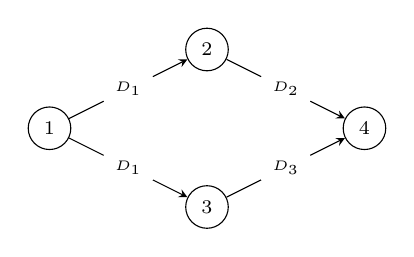
\begin{tikzpicture}
			\begin{scope}[every node/.style={circle,thin,draw}]
				\node (1a) at (+0+0,+0+0)	{\scriptsize $1$};
				\node (2a) at (+2+0,+1+0)	{\scriptsize $2$};
				\node (3a) at (+2+0,-1+0)	{\scriptsize $3$};
				\node (4a) at (+4+0,-0+0)	{\scriptsize $4$};
				
			\end{scope}

			\begin{scope}[>={stealth[black]},
				every node/.style={fill=white,circle},
				every edge/.style={draw=black,thin}]
				\path [->] (1a) edge node {\tiny $D_{1}$} (2a);
				\path [->] (1a) edge node {\tiny $D_{1}$} (3a);
				\path [->] (2a) edge node {\tiny $D_{2}$} (4a);
				\path [->] (3a) edge node {\tiny $D_{3}$} (4a);			
 			\end{scope}
		\end{tikzpicture}
		\subcaption{}
		\label{fig-STN}
	\end{subfigure}
	~
	\begin{subfigure}[b]{0.4\textwidth}
\begin{tikzpicture}
			\begin{scope}[->,>=stealth',shorten >=1pt,auto,
                semithick, scale = 1, transform shape,
                every node/.style={circle,thin,draw}]
				\node (z) at (-1.5,+1.5)	{\scriptsize $z$};
				
				\node (1a) at (+0+0,+0+0)	{\scriptsize $s_{1p}$};
				\node (2a) at (+2+0,+1+0)	{\scriptsize $s_{2p}$};
				\node (3a) at (+2+0,-1+0)	{\scriptsize $s_{3p}$};
				\node (4a) at (+4+0,-0+0)	{\scriptsize $s_{4p}$};
				
				\node (1b) at (+0+0.0,+0+3.0)	{\scriptsize $s_{1p'}$};
				\node (2b) at (+2+0.0,+1+3.0)	{\scriptsize $s_{2p'}$};
				\node (3b) at (+2+0.0,-1+3.0)	{\scriptsize $s_{3p'}$};
				\node (4b) at (+4+0.0,-0+3.0)	{\scriptsize $s_{4p'}$};				
			\end{scope}

			\begin{scope}[>={stealth[black]},
				every node/.style={fill=white,circle},
				every edge/.style={draw=black,thin}]
				
				% z1 arcs
				\path [<-] (z) edge[bend right=15] node {\tiny $0$} (1a);
				\path [->] (z) edge[bend left=15] node {\tiny $0$} (1a);
				\path [<-] (z) edge[bend right=15] node {\tiny $0$} (1b);
				\path [->] (z) edge[bend left=15] node {\tiny $0$} (1b);	
						
				% ij arcs for scenario p
				\path [<-] (1a) edge node {\tiny $-d_{1p}$} (2a);
				\path [<-] (1a) edge node {\tiny $-d_{1p}$} (3a);
				\path [<-] (2a) edge node {\tiny $-d_{2p}$} (4a);
				\path [<-] (3a) edge node {\tiny $-d_{3p}$} (4a);
				
				% ij arcs for scenario p'
				\path [<-] (1b) edge node {\tiny $-d_{1p'}$} (2b);
				\path [<-] (1b) edge node {\tiny $-d_{1p'}$} (3b);
				\path [<-] (2b) edge node {\tiny $-d_{2p'}$} (4b);
				\path [<-] (3b) edge node {\tiny $-d_{3p'}$} (4b);	

							
				% s1p - w - s1p'
				\path [->] (1a) edge[bend right=8] node[] {\tiny $w$} (1b);
				\path [<-] (1a) edge[bend left=8] node[] {\tiny $w$} (1b);
				
				% s2p - w - s2p'
				\path [dotted,<->] (2a) edge[bend left=15] node[pos=0.7] {\tiny $w$} (2b);
				
				% s3p - w - s3p'
				\path [dotted,<->] (3a) edge[bend right=15] node[pos=0.3] {\tiny $w$} (3b);
				
				% s4p - w - s4p'
				\path [->] (4a) edge[bend right=8] node[] {\tiny $w$} (4b);
				\path [<-] (4a) edge[bend left=8] node[] {\tiny $w$} (4b);
			\end{scope}
		\end{tikzpicture}
		\subcaption{}
		\label{fig-STN}
	\end{subfigure}

	\caption{Example task network (a) and resulting STP (b) for a sample $P=\{p, p''\}$.}
	\label{fig-STP}
\end{figure}

The \emph{earliest start time} (est) solution of any given STP (assuming it is consistent)
assigns to each variable the smallest value it may take over the set of feasible solutions.
Therefore,  the est solution of the resulting STP optimally solves $(P')$, leading us to the following observation.

\begin{obsv}
	By Lemma~\ref{lemm-Lambda}, an optimal solution $(s,t)$ for $(P)$ can be formed by finding the 
	earliest start time solution $s$ of the resulting STP and pairing it with $t$ formed by letting 
	$t_j = \max_{p\in \z{P}} s_{jp} - w$ for all $j$.
\end{obsv}

The est value of $s_{jp}$ is the length of the shortest-path (in the distance graph)
from (the node corresponding to) $s_{jp}$ to the special-purpose variable $z$ which is fixed to zero.
Those values can be found with a single-source shortest-path algorithm (e.g. Bellman-Ford \cite{pallottino1984})
in time $O(N M)$ where $N$ is the number of nodes and $M$ the number of arcs. 
In our case, $N=n m$ and $M = O(nm\delta)$, yielding $O(n^3m^2)$; already a better bound than that of solving $(P)$ as an LP.
However, in the following we obtain an even better bound with a dynamic programming algorithm.

\subsubsection{Computing the est solution by dynamic programming}
\begin{algorithm}[!t]
	\caption{Optimal release-times via dynamic programming}
 	\label{alg-main}
	\begin{algorithmic}[1]
		\State $l(s_{1p}) \leftarrow 0$ for all $p\in \z{P}$
		\For{each tier $j$ in a topological sort of $G(V,E)$}
			\State $k_{jp} \leftarrow \min \{l(s_{ip}) - d_{ip}: (i,j)\in E\}$ for all $p\in \z{P}$
			\State $p^* \leftarrow \arg \min \{k_{jp}: p \in \z{P}\}$ 
			\State $l(s_{jp}) \leftarrow \max \{k_{jp}, k_{jp^*} + w\}$ for all $p\in \z{P}$
		\EndFor
		\State $s_{jp} \leftarrow l(s_{jp})$ for all $j\in V, p\in\z{P}$
		\State $t_j \leftarrow \max_{p\in P} s_{jp} - w$ for each $j\in V$ 
	\end{algorithmic}
\end{algorithm}

Let us associate each task $j\in V$ with a corresponding \emph{tier} including all nodes $\{s_{jp}: p \in \z{P}\}$ 
of the STP distance graph.
A few remarks on the structure of the STP are in order.
First, due to (\ref{P'-pp}) the resulting STP is not acyclic, but each cycle only includes nodes that belong to the same tier.
Second, due to (\ref{P'-sisj}) there is a path from each node in tier $j$ to each node in tier $i$ if and only if there is a path from task $i$ to $j$ in $G(V, E)$.

%To form the est solution, we want to compute the shortest-path from each node $s_{jp}$ to special-purpose node $z$.
Let $l(s_{jp})$ denote the shortest-path length from $s_{jp}$ to $z$ (i.e. the value of variable $s_{jp}$ in an optimal solution of $(P')$).
From the structure of the resulting STP, we have:
\begin{align}
	l(s_{jp}) = \min\left\{
		\min_{(i,j)\in E} (l(s_{ip}) - d_{ip}), \min_{p' \neq p} l(s_{jp'}) + w
	\right\}
	\label{def-lsjp}
\end{align}

The existence of cycles complicates solving subproblem $l(s_{jp})$
as it depends on (and is a dependency of) other subproblems $l(s_{jp'})$ in the same tier.
However, we can ``break'' dependencies between subproblems in the same tier as shown below.

Define $k_{jp} := \min_{(i,j)\in E} (l(s_{ip}) - d_{ip})$ and $p^* := \arg \min_{p\in \z{P}} k_{jp}$.
\begin{lemm}
	$l(s_{jp}) = \min\{k_{jp}, k_{jp^*} + w\}$
\begin{proof}
	Begin by noting that the shortest-path from $s_{jp}$ to $z$ visits at most one node $s_{jp'}$ from the same tier.
	As such, for every $s_{jp}$ we have that: either $l(s_{jp}) = k_{jp}$, or $l(s_{jp}) = k_{jp'} + w < k_{jp}$ for some $p' \neq p$.

	Now, note that $l(s_{jp^*}) = k_{jp^*}$,
	since if not (i.e. if $l(s_{jp^*}) \neq k_{jp^*}$),
	then $l(s_{jp^*}) = k_{jp'} + w < k_{jp^*}$ with $p'\neq p^*$, which contradicts the definition of $p^*$.

	Last, we show that if $l(s_{jp}) \neq k_{jp}$ then $l(s_{jp}) = k_{jp^*} + w$.
	Suppose not.
	Since $l(s_{jp}) \neq k_{jp}$ then according to (\ref{def-lsjp}), $l(s_{jp}) = l(s_{jp'}) + w$ but with $p' \neq p^*$.
	Expanding $l(s_{jp'})$ according to (\ref{def-lsjp}),
	\begin{align*}
		\min\{k_{jp'}, \min_{p''\neq p'} l(s_{jp''}) + w\} + w  < l(s_{jp^*}) + w = k_{jp^*} + w
	\end{align*}
	and since $k_{jp'} \geq k_{jp^*}$,
	\begin{align*}
		\min_{p''\neq p'} l(s_{jp''}) + w < k_{jp^*} \\ \Leftrightarrow
		l(s_{jp^*}) + w < k_{jp^*}
	\end{align*}
	which contradicts that $l(s_{jp^*}) = k_{jp^*}$.
\end{proof}
\end{lemm}

The resulting recursion suggests a dynamic programming approach, summarized in Algorithm~\ref{alg-main}.
It involves solving the subproblems of one tier at a time,
visiting tiers according to a topological sort of $G(V,E)$ (recall that tiers correspond to tasks $j\in V$).
Finding a topological sort takes $O(n\delta)$ \cite{tarjan1976},
recalling that $\delta$ denotes the max in-degree of a task in the network.
The overall complexity of Algorithm~\ref{alg-main} is therefore $O(nm\delta) \subseteq O(n^2m)$.
